% Copyright 2022 Fausto Spoto
%
% Licensed under the Apache License, Version 2.0 (the "License");
% you may not use this file except in compliance with the License.
% You may obtain a copy of the License at
%
%    http://www.apache.org/licenses/LICENSE-2.0
%
% Unless required by applicable law or agreed to in writing, software
% distributed under the License is distributed on an "AS IS" BASIS,
% WITHOUT WARRANTIES OR CONDITIONS OF ANY KIND, either express or implied.
% See the License for the specific language governing permissions and
% limitations under the License.

\documentclass[11pt]{beamer}  %% versione proiettore
%%\documentclass[11pt,handout]{beamer} %% versione stampa
\usepackage{lucidiJb-2ed}

\usepackage{relsize}

\mode<article>
{
  \usepackage{fullpage}
  \usepackage{hyperref}
}

\mode<presentation>
{
  \setbeamertemplate{background canvas}[vertical shading][bottom=red!10,top=blue!10]
  \usetheme{Course}
  \usefonttheme[onlysmall]{structurebold}
}

\subtitle{Blockchain Technology}
\title{Introduction}
\institute{Universit\`a di Verona, Italy}
\date{November 2022}

\setbeamercovered{invisible}

\def\codesize{\smaller}
\def\<#1>{\codeid{#1}}
\newcommand{\codeid}[1]{\ifmmode{\mbox{\codesize\ttfamily{#1}}}\else{\codesize\ttfamily #1}\fi}

\begin{document}

\begin{frame}
  \titlepage
\end{frame}

\begin{frame}\frametitle{The mainstream view of blockchain}

  \begin{center}
    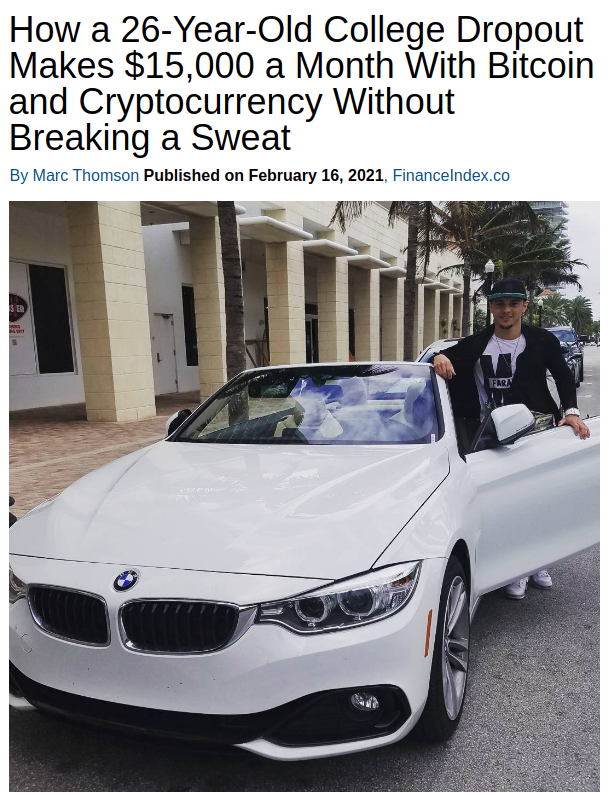
\includegraphics[scale=0.209,clip=false]{pictures/dropout.png}
    \hspace*{2ex}
    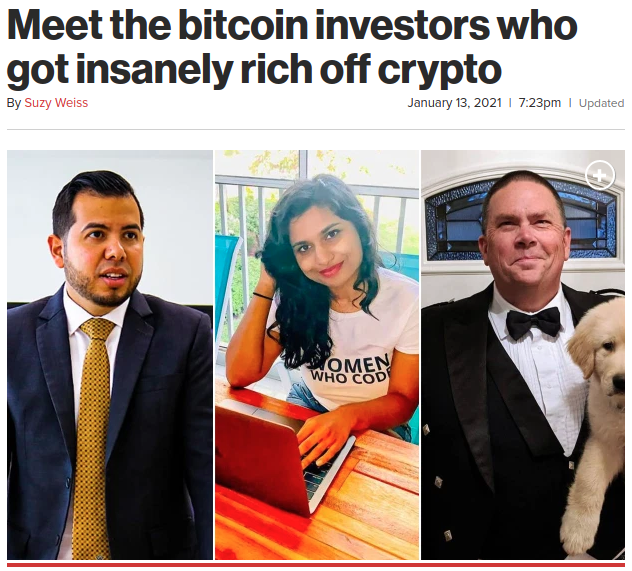
\includegraphics[scale=0.29,clip=false]{pictures/insane.png}
  \end{center}

\end{frame}

\begin{frame}\frametitle{The mainstream view of blockchain}

  \begin{center}
    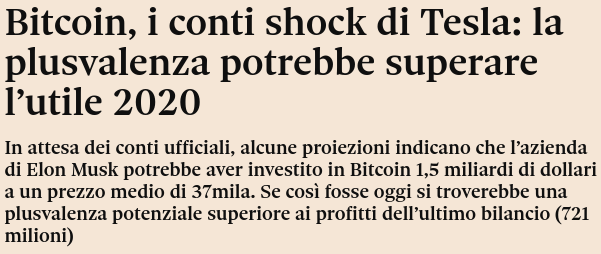
\includegraphics[scale=0.4,clip=false]{pictures/tesla.png}
  \end{center}

\end{frame}

\begin{frame}\frametitle{History}

  \begin{itemize}
  \item[1988] proof-of-work (Dwork \& Naor)
  \item[1991] a cryptographically secure chain of blocks (Haber \& Stornetta)
  \item[199x] smart contracts (Szabo)
  \item[2008] Bitcoin (Nakamoto)
  \item[2012] proof-of-stake (Peercoin)
  \item[2013] Ethereum (Buterin \& Wood)
  \item[2014] Tendermint generic proof-of-stake engine (Kwon)
  \item[2022] Ethereum 2.0 adopts the proof-of-stake
  \end{itemize}
  
\end{frame}

\begin{frame}\frametitle{Distributed network}

  \begin{center}
    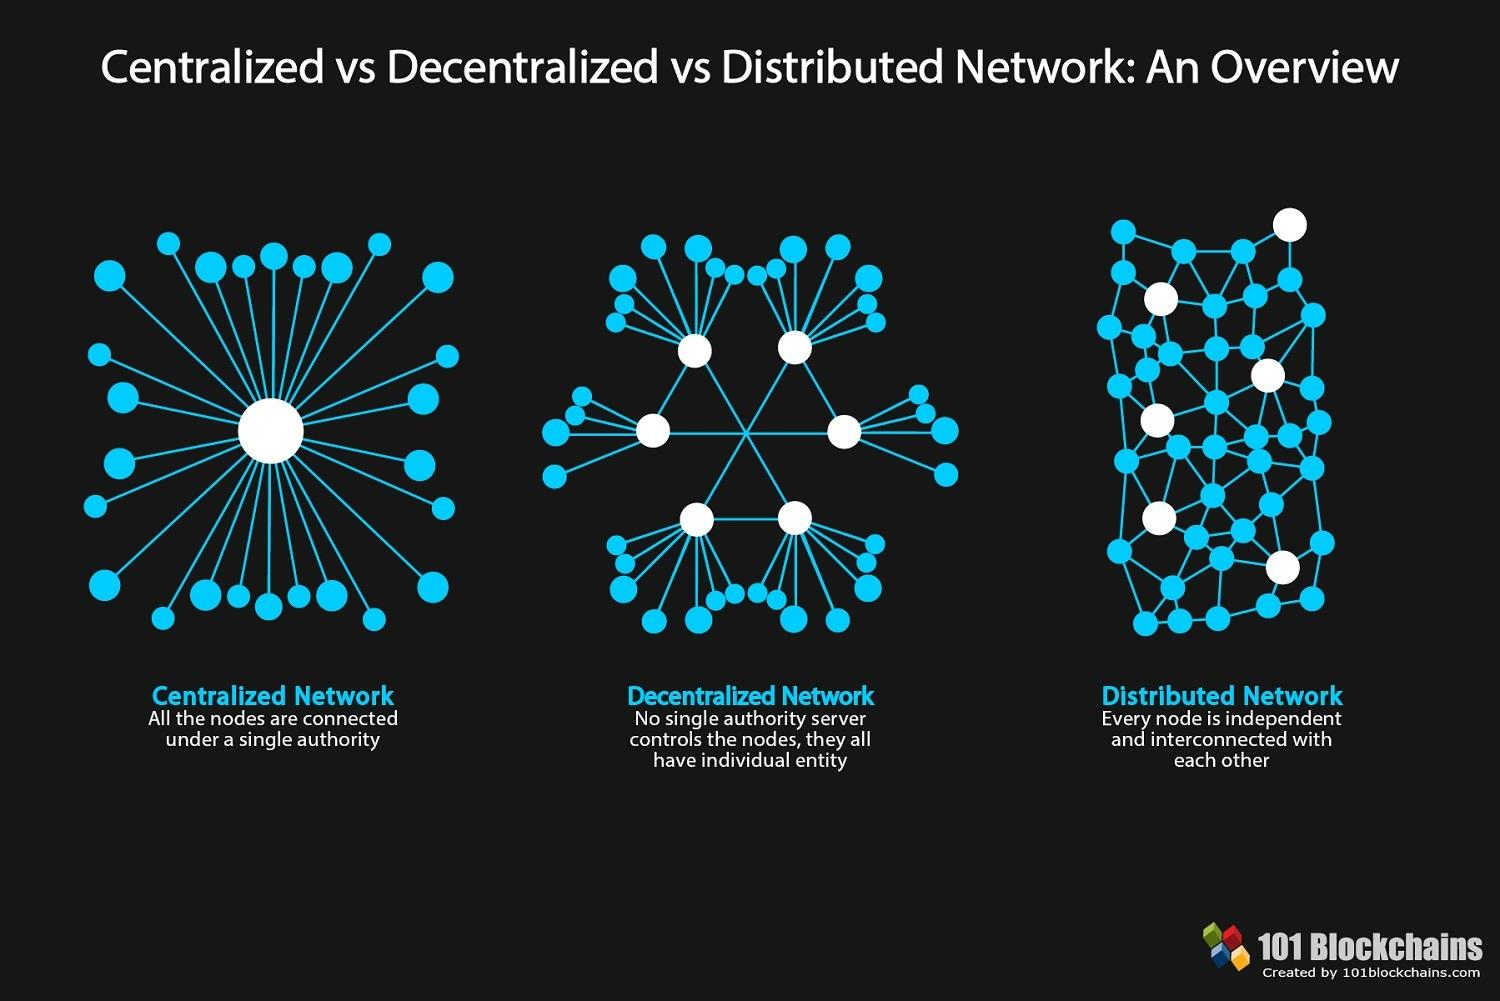
\includegraphics[scale=0.22,clip=false]{pictures/distributed.jpg}
  \end{center}

\end{frame}

\begin{frame}\frametitle{Cryptocurrencies}

  \begin{center}
    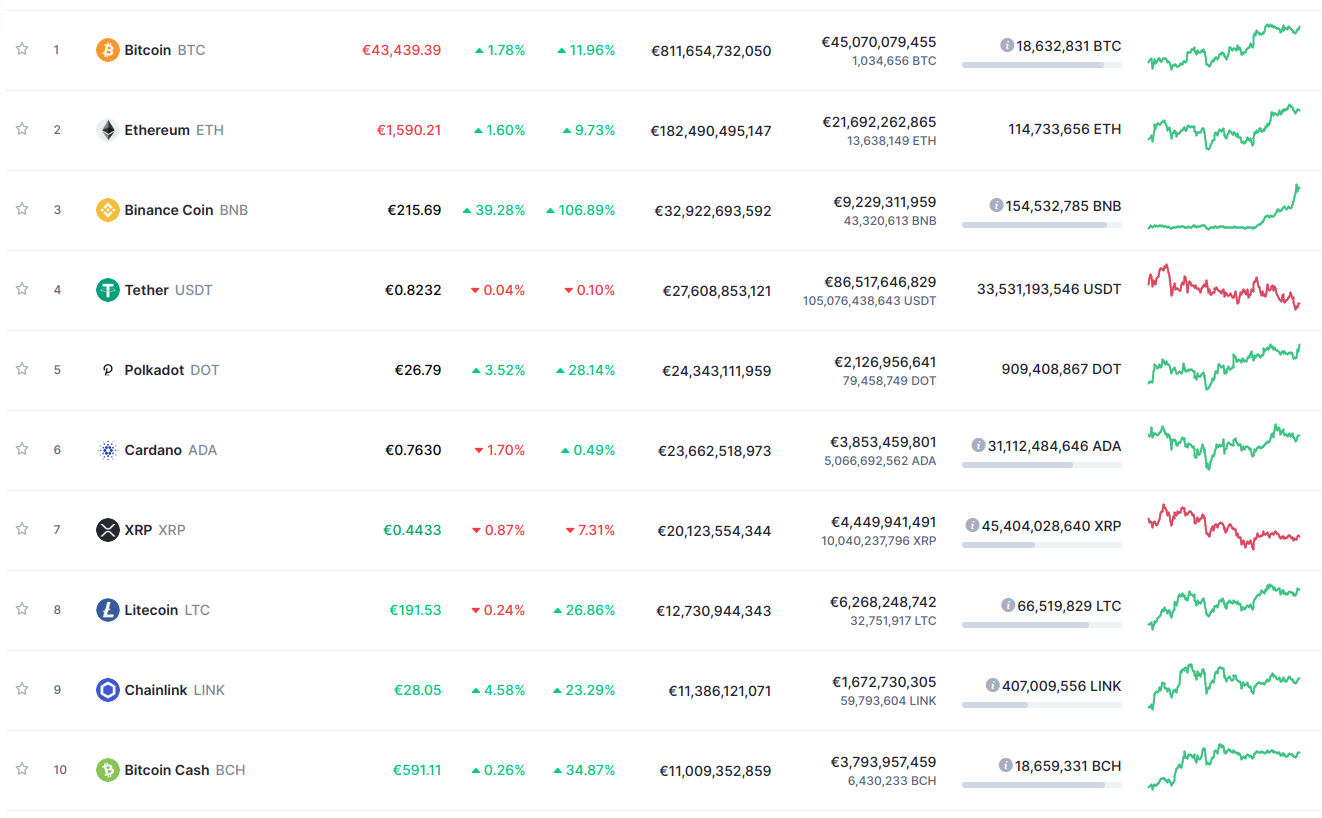
\includegraphics[scale=0.258,clip=false]{pictures/market.png}
  \end{center}

\end{frame}

\begin{frame}\frametitle{Bitcoin chart}

  \begin{center}
    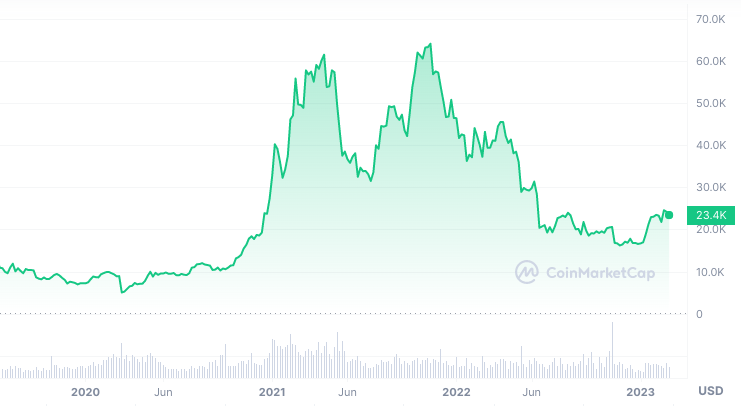
\includegraphics[width=\textwidth,clip=false]{pictures/bitcoin-coinmarketcap.png}
  \end{center}

\end{frame}

\begin{frame}\frametitle{Bitcoin capitalization (2018)}

  \begin{center}
    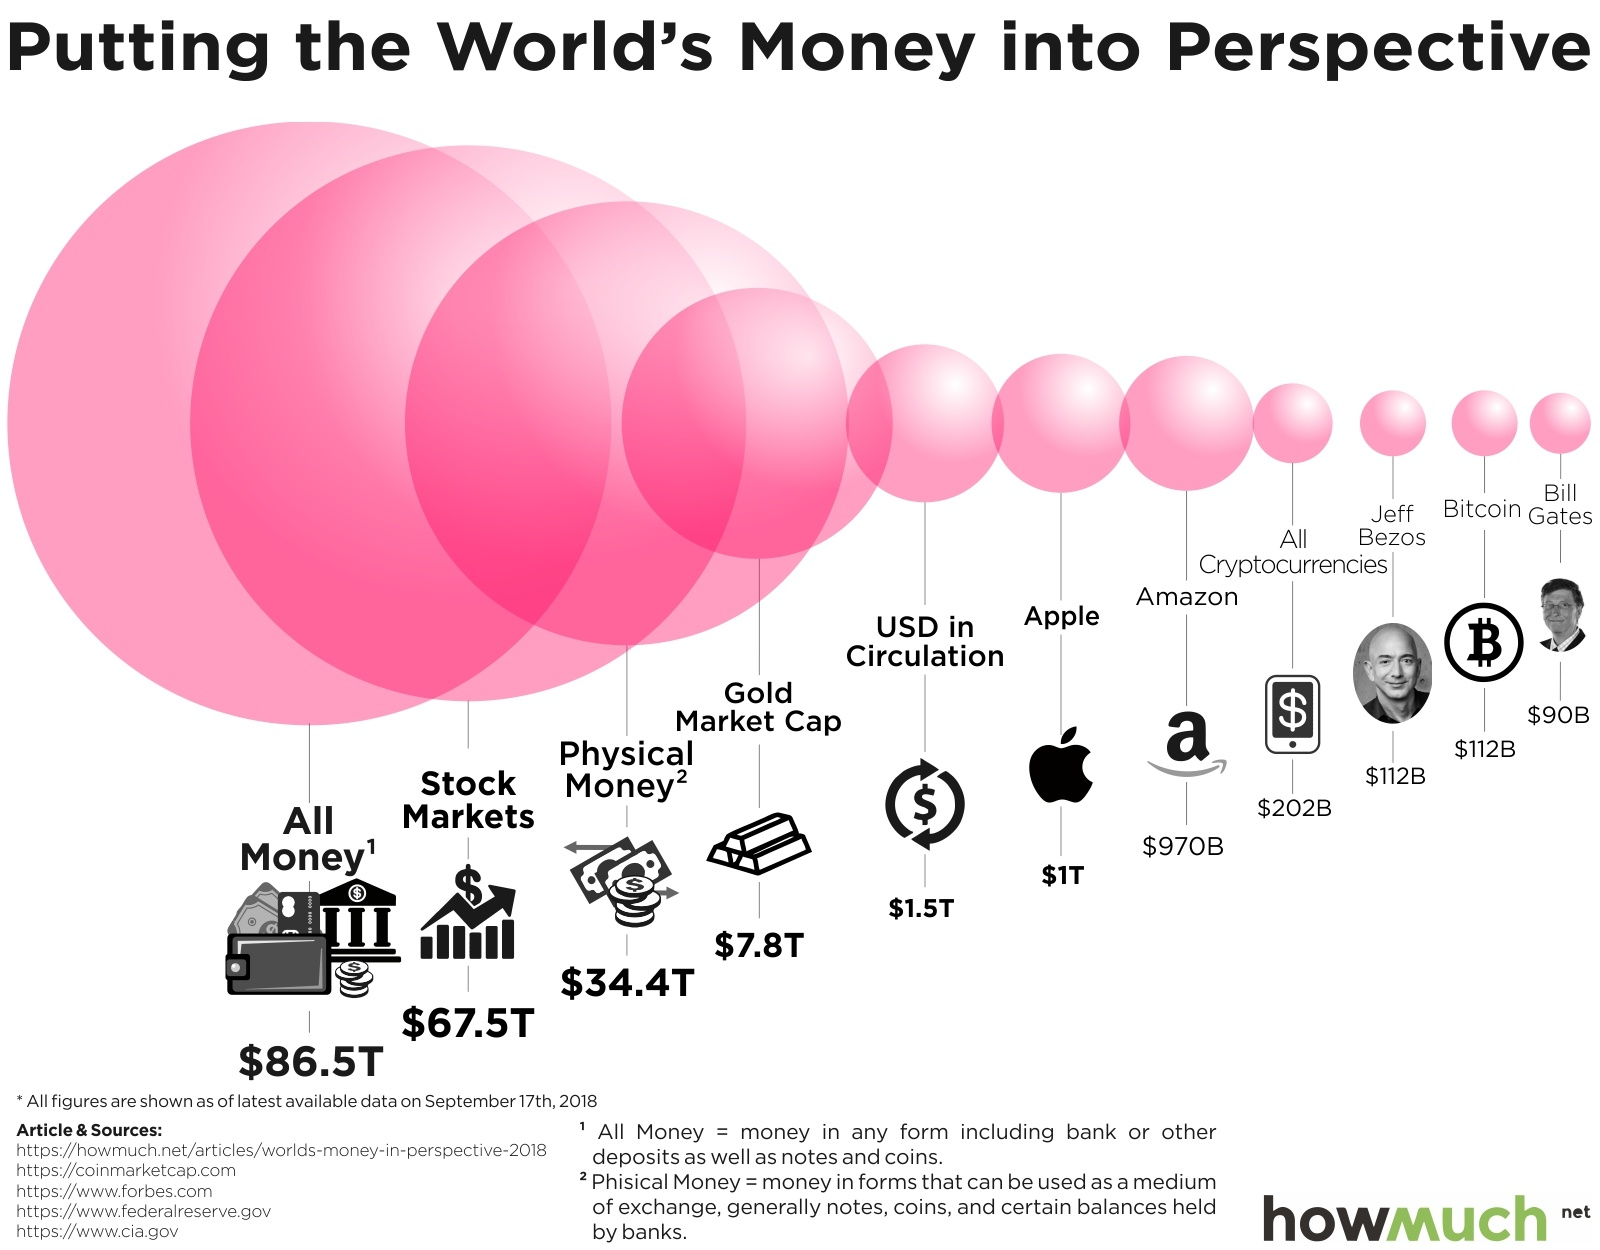
\includegraphics[scale=0.16,clip=false]{pictures/bitcoin-capitalization.jpg}
  \end{center}

  \begin{center}
    source: \url{HowMuch.net}, a financial literacy website
  \end{center}

\end{frame}

\begin{frame}\frametitle{Bitcoin transactions}

  \begin{center}
    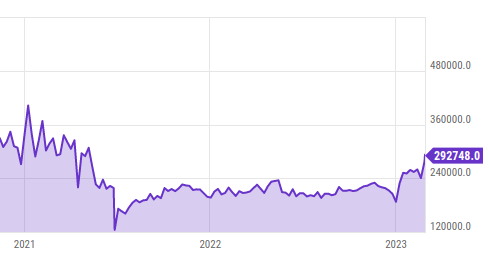
\includegraphics[scale=0.3,clip=false]{pictures/bitcoin-daily.png}
  \end{center}

  \begin{center}
    Around 300,000 transactions per day
  \end{center}

\end{frame}

\begin{frame}\frametitle{Credit cards transactions (billions, 2018)}

  \begin{center}
    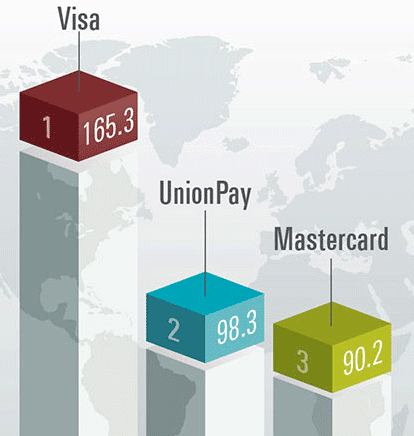
\includegraphics[scale=0.3,clip=false]{pictures/credit-cards.png}
  \end{center}

  \begin{center}
    Visa: around 451,639,000 transactions per day\\
    UnionPay: around 268,579,000 transactions per day\\
    Mastercard: around 246,448,000 transactions per day\\
    Bitcoin: around 300,000 transactions per day
  \end{center}

\end{frame}

\begin{frame}\frametitle{Bitcoin transaction fees}

  \begin{center}
    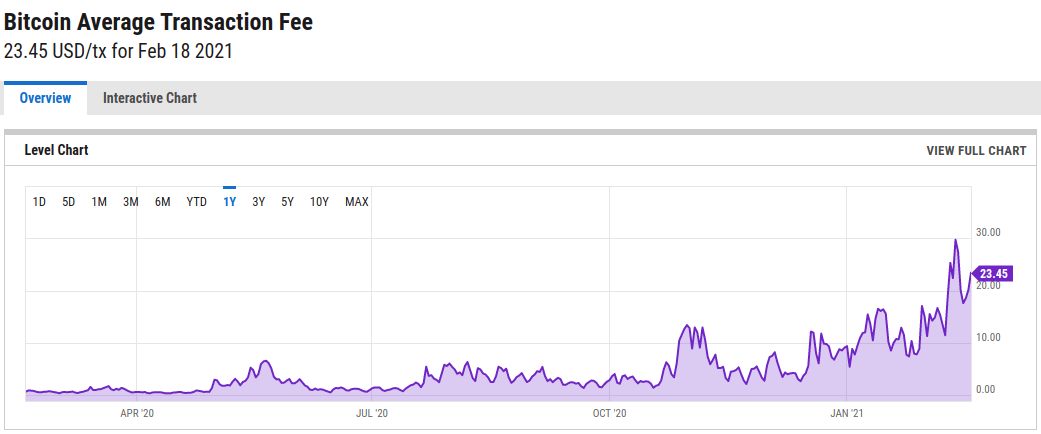
\includegraphics[width=\textwidth,clip=false]{pictures/bitcoin-fees.png}
  \end{center}

  \begin{center}
    Independent from the transacted value
  \end{center}

\end{frame}

\begin{frame}\frametitle{Credit cards transaction fees}

  \begin{center}
    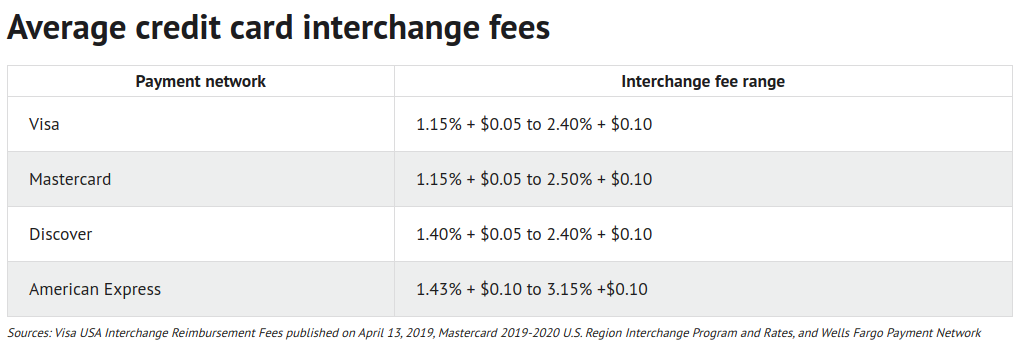
\includegraphics[width=\textwidth,clip=false]{pictures/credit-cards-fees.png}
  \end{center}

  \begin{center}
    Proportional to the transacted value
  \end{center}

\end{frame}

\begin{frame}\frametitle{Bitcoin as a web service}

  \begin{center}
    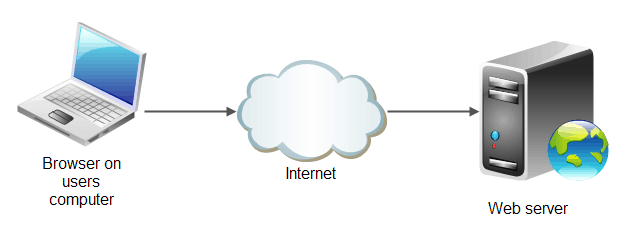
\includegraphics[scale=.3,clip=false]{pictures/web-server.png}
  \end{center}

  \medskip

  The server keeps a map (\alert{ledger}) $\mathit{user\_id}\Rightarrow\mathit{balance}$
  and accepts transactions to transfer balances

  \medskip

  Users interact through a browser (\alert{wallet}) to ask to transfer balances

  \medskip
  The server is actually a worldwide peer-to-peer (p2p) network of computers

  \begin{center}
    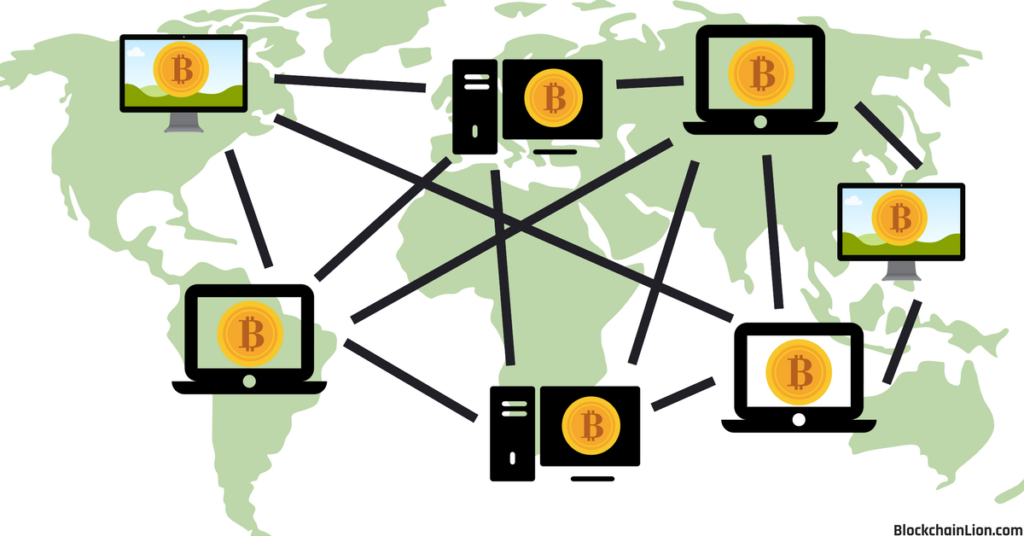
\includegraphics[scale=.13,clip=false]{pictures/distributed.png}
  \end{center}

\end{frame}

\begin{frame}\frametitle{Headers, blocks and blockchain, genesis block}

  \begin{center}
    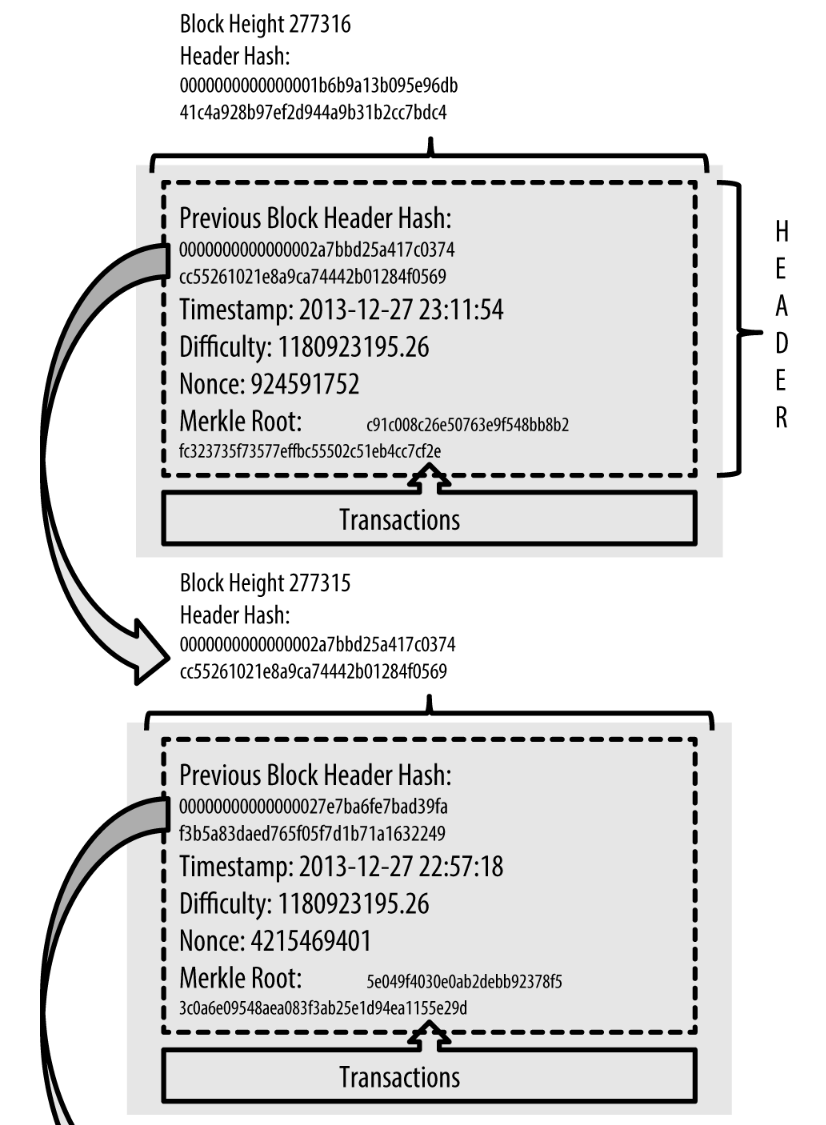
\includegraphics[scale=0.2,clip=false]{pictures/bitcoin-blocks.png}
  \end{center}

\end{frame}

\begin{frame}\frametitle{The magic behind the Proof of Work}

  \begin{greenbox}{}
    It makes expensive the production of new blocks, in time and cost (electricity)
    \begin{itemize}
    \item who produces invalid blocks sees its blocks rejected by peers and wastes resources
    \item a single node cannot drive the history, since it must fight against
      the hashing power of all other nodes together
    \item forks become unlikely, since the probability of finding a new block at the same time
      is small
    \end{itemize}
  \end{greenbox}

\end{frame}

\begin{frame}\frametitle{PoW costs electricity}

  \begin{greenbox}{2019}
    \begin{center}
      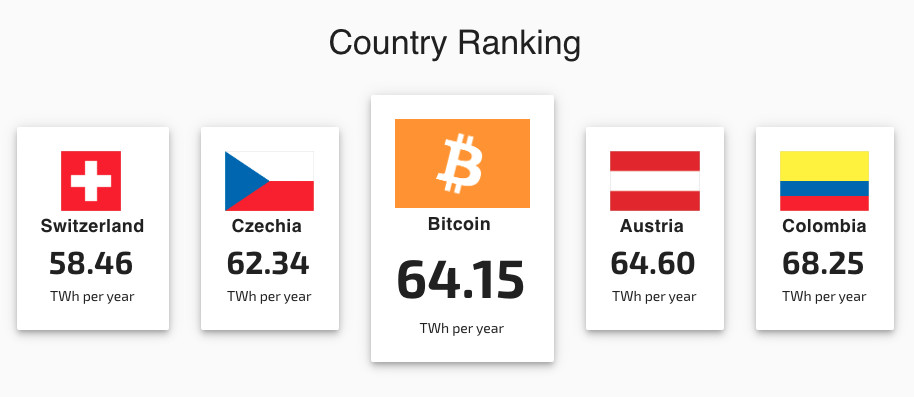
\includegraphics[scale=0.17,clip=false]{pictures/bitcoin-consumption.jpg}
      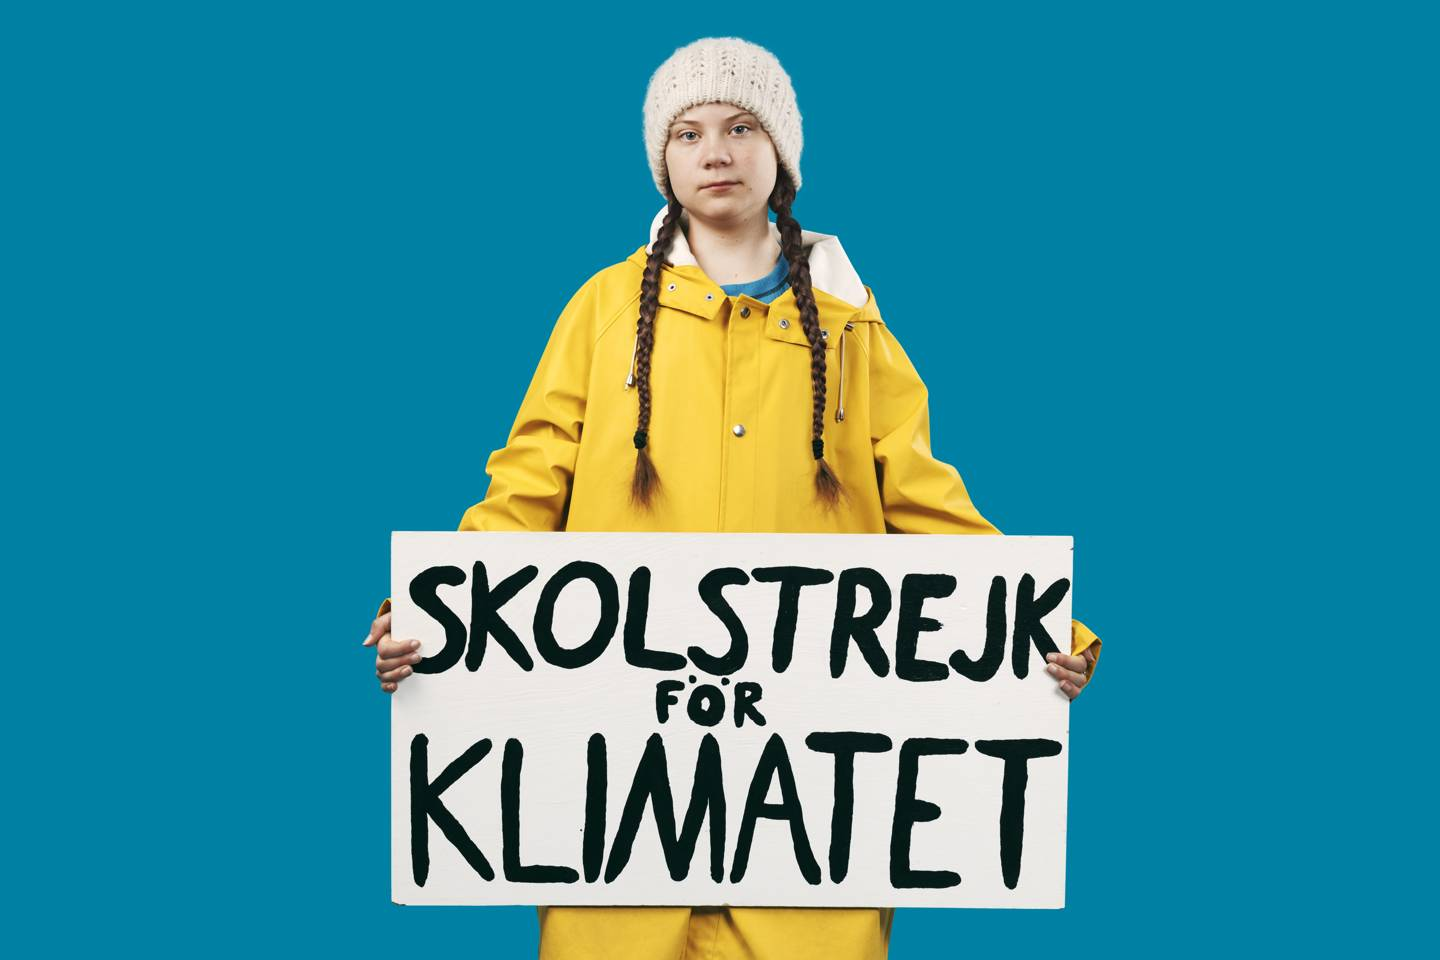
\includegraphics[scale=0.14,clip=false]{pictures/greta.jpg}
    \end{center}
  \end{greenbox}
    
\end{frame}

\begin{frame}\frametitle{Consensus attacks}

  \begin{greenbox}{Two main categories}
    \begin{enumerate}
    \item history change (for the topmost few blocks)
    \item denial-of-service (against specific transactions or accounts)
    \end{enumerate}
  \end{greenbox}

  \bigskip

  Possible if the attacker controls a large portion of the total hashing power

  \begin{center}
    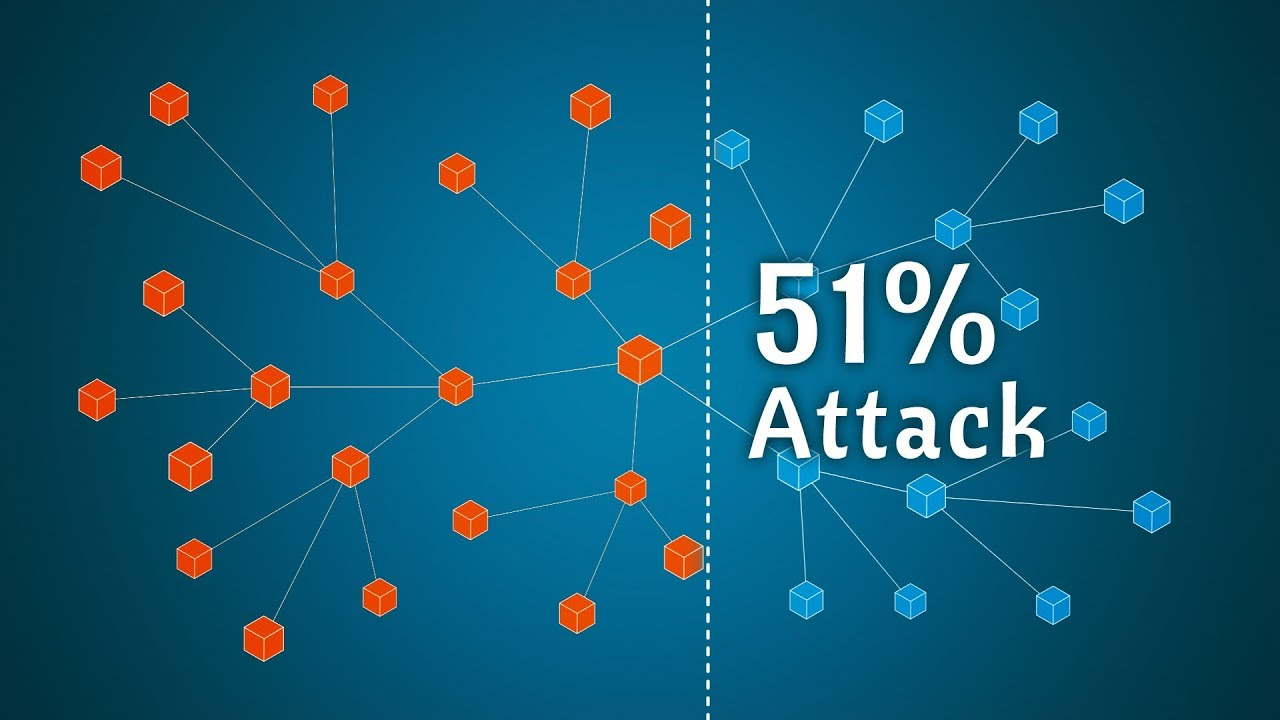
\includegraphics[scale=0.17,clip=false]{pictures/51-percenters.jpg}
  \end{center}

\end{frame}

\begin{frame}\frametitle{How the 51\% attack works}

  \begin{greenbox}{The malicious miner spends $100$ BTC on the public chain
      while it is adding blocks to its
      private blockchain, without broadcasting them. In its private chain,
      the spend transaction is missing}
    \begin{center}
      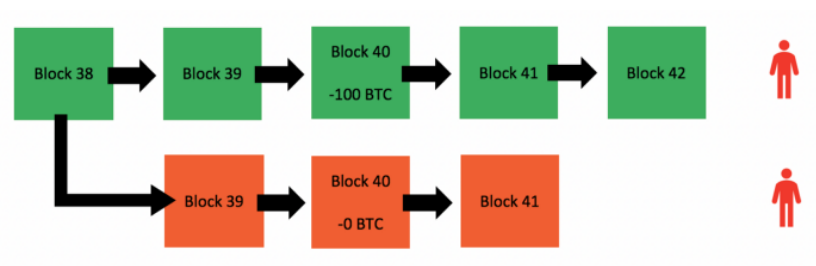
\includegraphics[width=\textwidth,clip=false]{pictures/51attack_1.png}
    \end{center}
  \end{greenbox}

\end{frame}

\begin{frame}\frametitle{How the 51\% attack works}

  \begin{greenbox}{The malicious miner makes its private chain longer,
      since it has more hashing power than the rest of the miners taken together}
  \begin{center}
    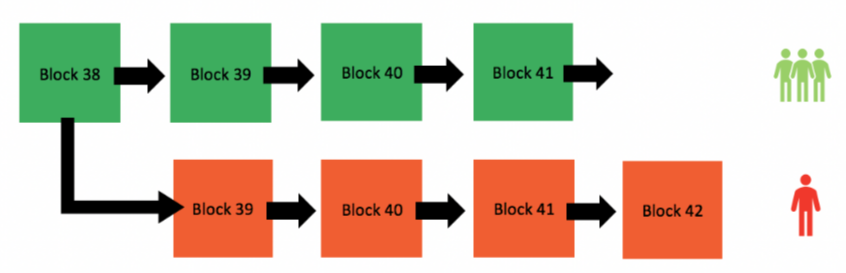
\includegraphics[width=\textwidth,clip=false]{pictures/51attack_2.png}
  \end{center}
  \end{greenbox}

\end{frame}

\begin{frame}\frametitle{How the 51\% attack works}

  \begin{greenbox}{The malicious miner broadcasts its private chain; since it is longer,
      all other miners switch to this alternative view of the history}
  \begin{center}
    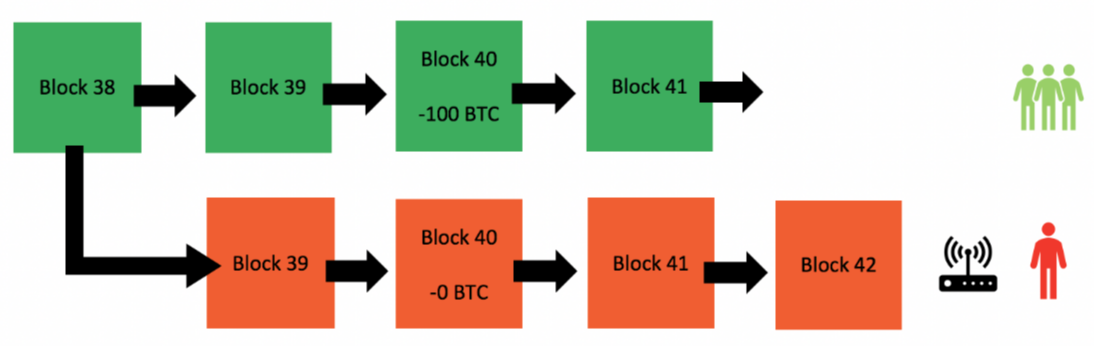
\includegraphics[width=\textwidth,clip=false]{pictures/51attack_3.png}
  \end{center}
  \end{greenbox}

\end{frame}

\begin{frame}\frametitle{How the 51\% attack works}

  \begin{greenbox}{The malicious miner can spend its $100$ BTC again! Everybody agrees\ldots}
  \begin{center}
    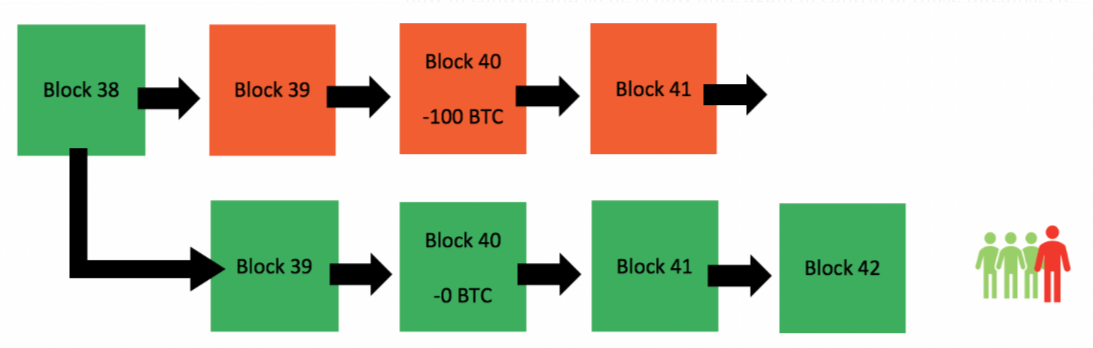
\includegraphics[width=\textwidth,clip=false]{pictures/51attack_4.png}
  \end{center}
  \end{greenbox}

  \bigskip

  \begin{center}
    History is written by the victors
  \end{center}

\end{frame}

\begin{frame}\frametitle{Bitcoin has probabilistic finality}

  \begin{center}
    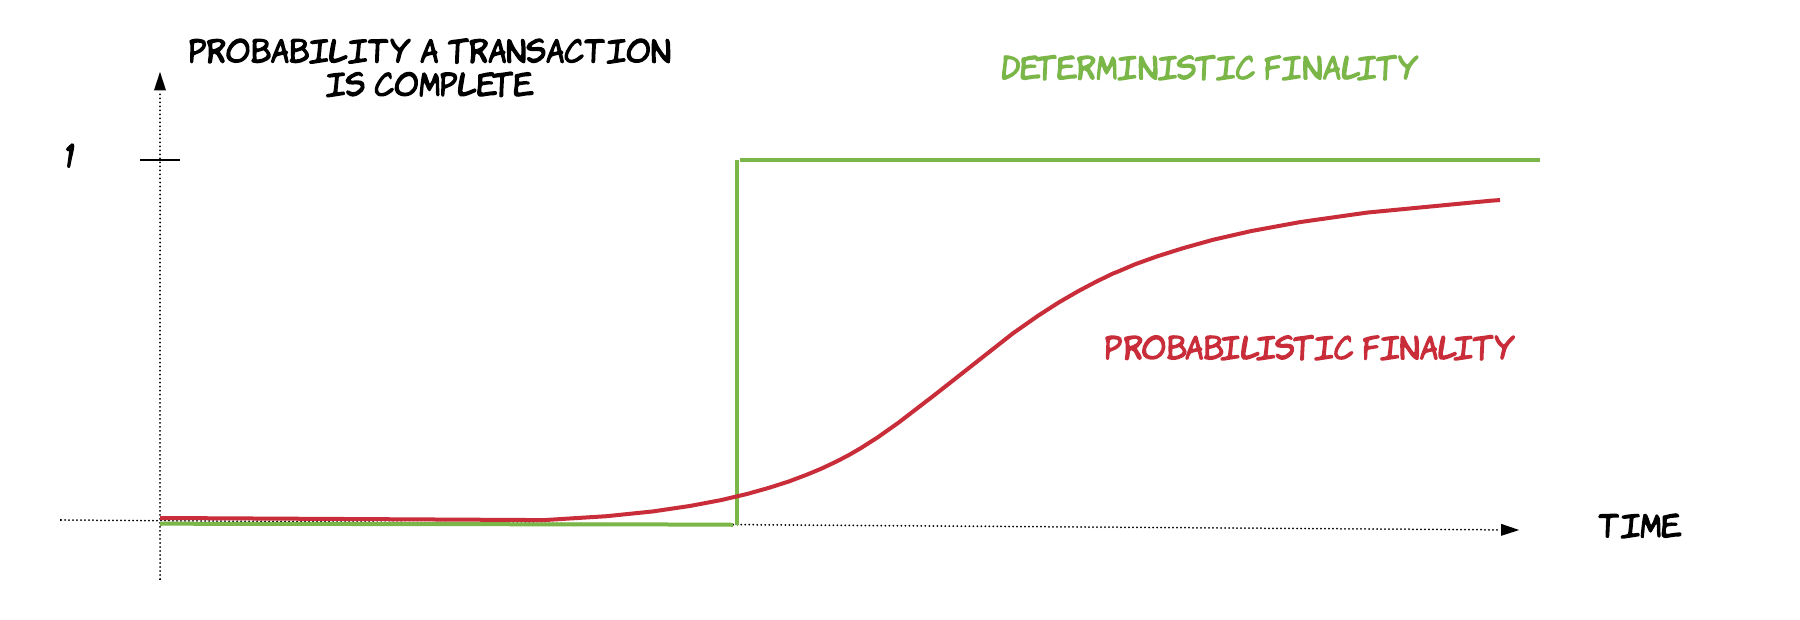
\includegraphics[width=\textwidth,clip=false]{pictures/finality.png}
  \end{center}

\end{frame}

\begin{frame}\frametitle{The hype cycle}

  \begin{center}
    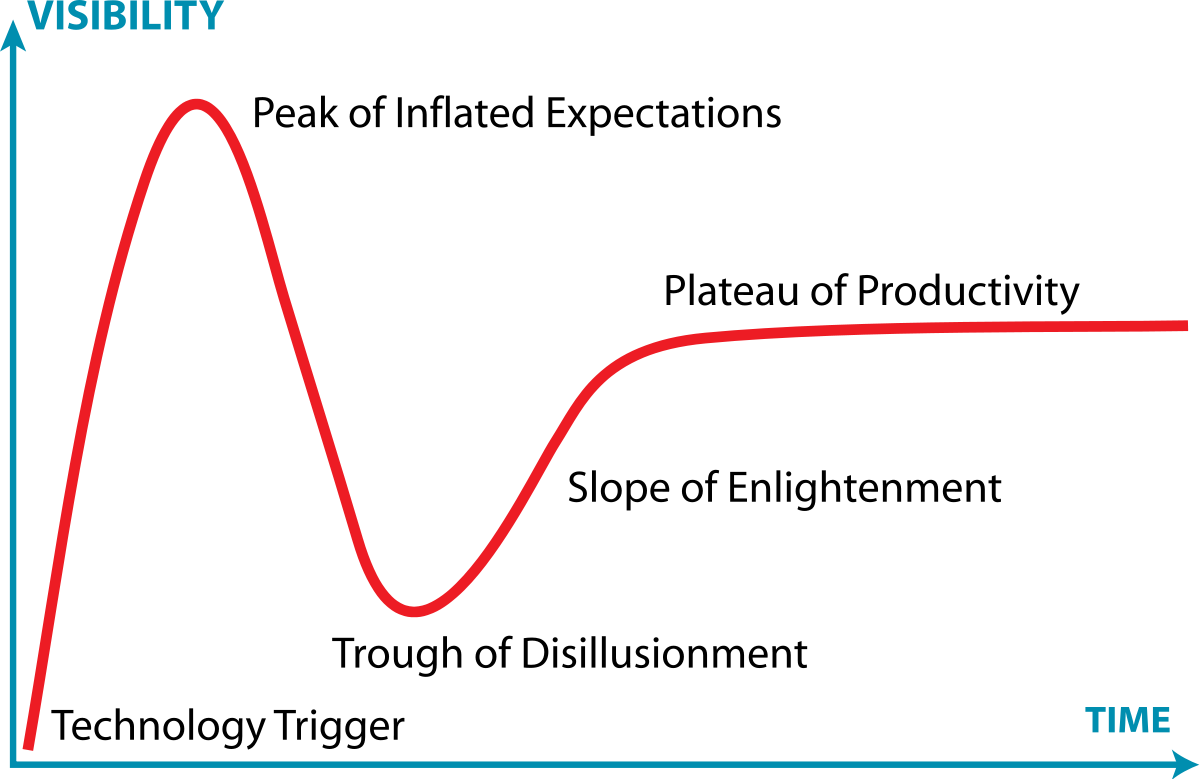
\includegraphics[width=\textwidth,clip=false]{pictures/hype-cycle.png}
  \end{center}

\end{frame}

\begin{frame}\frametitle{Beyond the hype}

  \begin{center}
    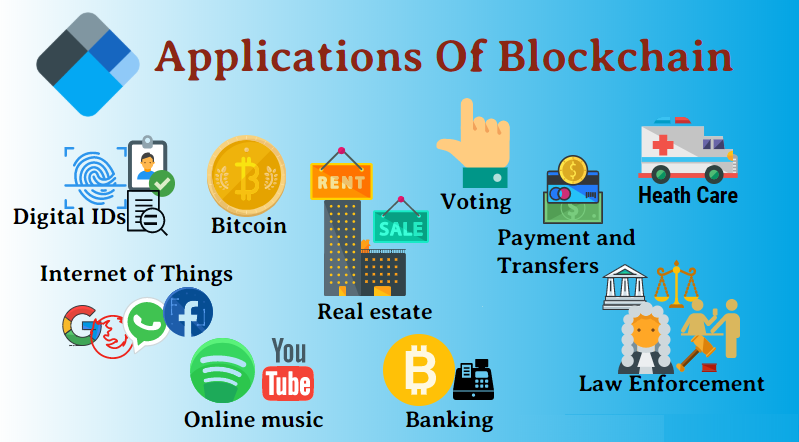
\includegraphics[scale=0.4,clip=false]{pictures/blockchain-applications.png}
  \end{center}

\end{frame}

\begin{frame}\frametitle{Beyond the hype}

  \begin{center}
    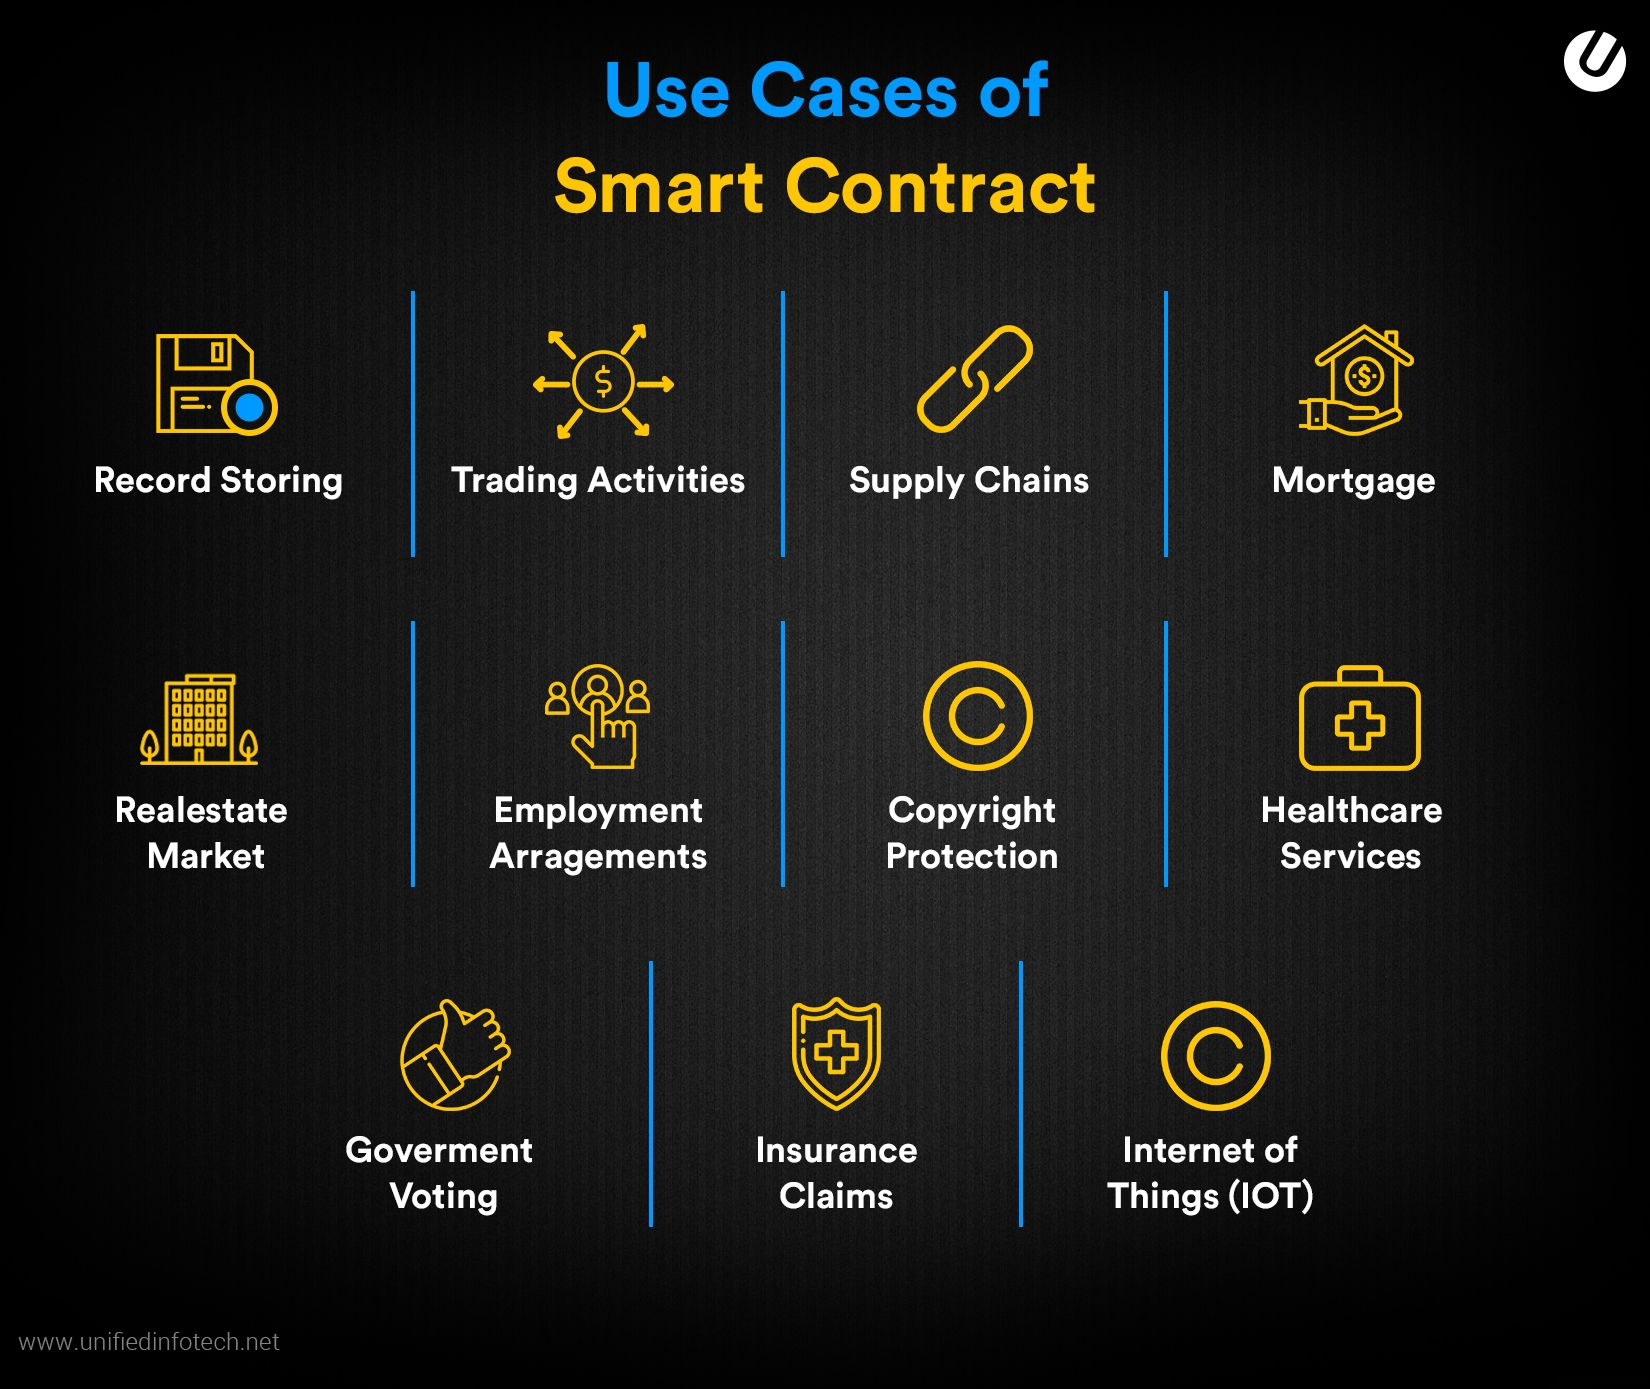
\includegraphics[scale=0.16,clip=false]{pictures/smart-contract-applications.jpg}
  \end{center}

\end{frame}

\begin{frame}\frametitle{Future trends}

  \begin{itemize}
  \item \alert{\url{https://ipfs.io}}: decentralized file storage
  \item \alert{\url{https://identity.foundation}}: decentralized identity
  \item \alert{\url{https://defipulse.com}}: decentralized finance (DeFi)
  \item \alert{\url{https://pkt.cash}}: decentralized internet service providers
  \item integration with the internet of things
  \end{itemize}

  \begin{center}
    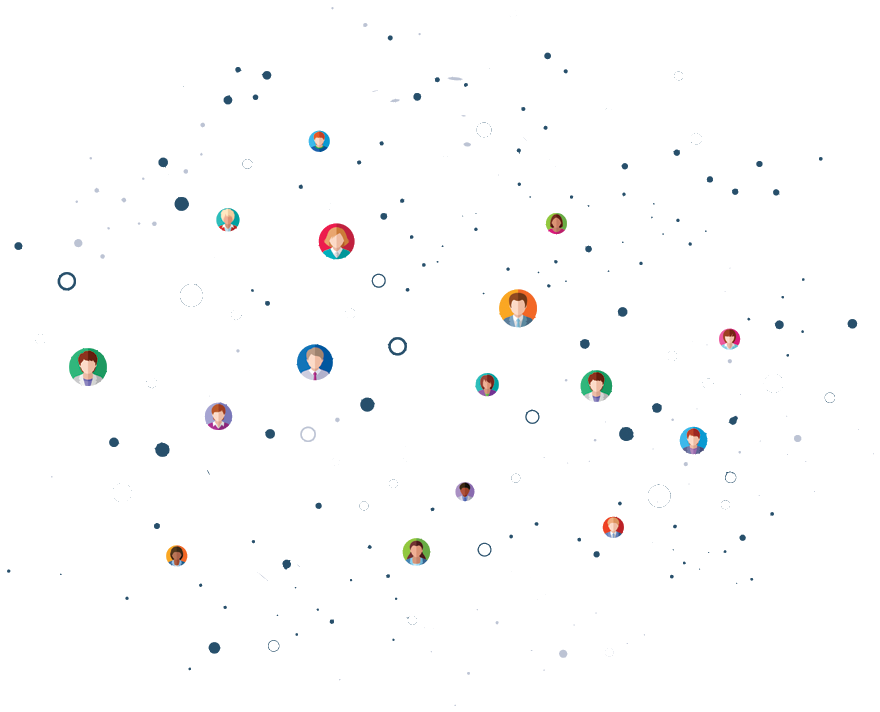
\includegraphics[scale=0.16,clip=false]{pictures/did.png}
  \end{center}

\end{frame}

\begin{frame}\frametitle{NFT}

  \begin{center}
    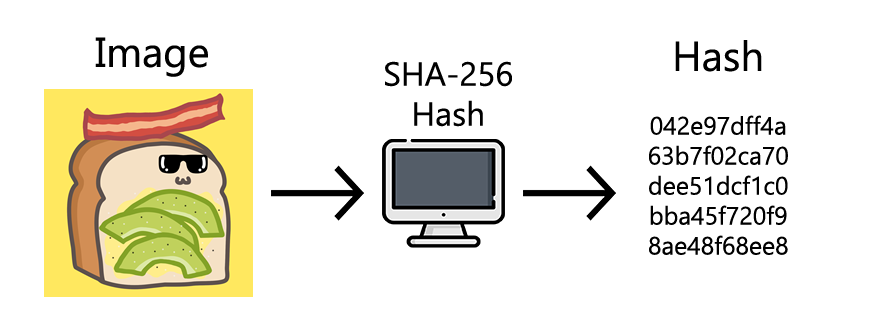
\includegraphics[scale=0.4,clip=false]{pictures/hash.png}
  \end{center}
\end{frame}

\begin{frame}\frametitle{Vero4Chain}
  \begin{center}
    
\includegraphics[scale=0.6,clip=false]{pictures/vero4chain.png}\\
    \url{https://www.vero4chain.it}
  \end{center}

  \begin{itemize}
  \item spin-off company of the University of Verona
  \item provides software and services for blockchain
  \item currently offering stages in the area of
    software development for web applications connected to
    blockchains
  \end{itemize}
\end{frame}

\end{document}
